\section{Future Work}\label{sec:future}

  The scope of what is possible to achieve in this project is far beyond what a
  single individual could accomplish in one year. There are many ideas and
  concepts that came up during this project that were identified as being
  valuable to accomplish in future iterations. This section lists some of those
  that the developer plans to implement going forward.

  \subsection{Meson Build System}\label{sec:future-meson}

    The Autotools build system is somewhat complex and difficult to maintain.
    More modern build systems have emerged such as \texttt{waf} and
    \testtt{meson} that would likely provide a much easier system for new
    contributors to modify as well as improve on the time required to perform a
    build.

    Objectives:

    \begin{itemize}
      \item Reduce build time
      \item Simplify additions and modifications to the build system
      \item Reduce build system dependencies in Continuous Integration
      \item Improve readability of build configurations
    \end{itemize}

    This graphic taken from \url{http://mesonbuild.com/Simple-comparison.html}
    shows the performance comparisons of different build systems. While not the
    fastest of the options, it is comparably simpler to develop for than CMake
    and Premake.

    \begin{figure}[H]
      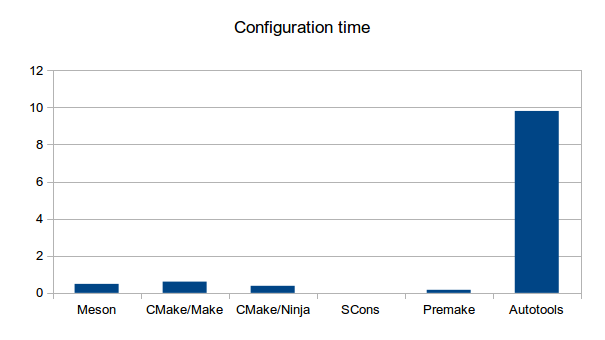
\includegraphics[width=\textwidth]{figures/future/conftime}
      \caption{Performance Comparison of Build Systems}
      \label{fig:fut-meson-perf}
    \end{figure}

  \subsection{Plugin Generator}\label{sec:future-plugin-generator}

    The Peas library for plugins was used heavily in the development of this
    project to keep all services modular. While Peas does make it significantly
    simpler to add plugins to a system it can still require a reasonable amount
    of setup that includes the connection to the various service add-ins and
    providers, a build system that results in plugins being located in the
    correct location, and knowledge of the four different types of plugins
    available to developers.

    A utility application to automate this project could be created that uses
    templates, and has a simple well design CLI that queries the developer/user
    for what they want to bootstrap.

    Objectives:

    \begin{itemize}
      \item Simplify and automate the plugin development process
      \item Eliminate errors in creating plugins
      \item Reduce the amount of knowledge a developer requires to contribute
    \end{itemize}

  \subsection{GUI Integration}\label{sec:future-gui}

    One of the main existing components of the software that OpenDCS was ported
    from is a GUI application that does all of the tasks that were split out
    into separate services, albeit not as well. Another desirable addition to
    this project would be modifying the existing GUI application, refactored as
    \emph{dcsg}, to receive data from the services to use with the dashboards
    that can be created for system operators.

    This project would involve integrating service data receivers in the form
    of stream subscribing sockets, as well as service queries performed using
    a request/reply pair. It would also be necessary to document how the GUI
    can be integrated with the data coming from the services for dashboard
    designers as it would add a layer of complexity that they are currently
    not encumbered by.

    Objectives:

    \begin{itemize}
      \item Increase the availability of measurement data by communicating with
        multiple sources
      \item Increase data logging options from the GUI without needing to modify
        the source code of that project
      \item Decouple the GUI from fundamental operations of a data acquisition
        system
    \end{itemize}

  \subsection{ZeroMQ Traffic Encryption}\label{sec:future-czmq}

    ZeroMQ was used throughout this project to communicate data among services,
    this library is developed in C++ and its API accessed through a C wrapper.
    The wrapper used was a vanilla implementation and only provides basic
    socket types and communication schemes. A higher level C library exists to
    interoperate with ZeroMQ by the name of CZMQ, this library binding offers
    other useful features in addition to the core socket and messaging API
    available in the one currently in use, these include mechanisms for
    authentication and encryption, generic message containers, and the ability
    to perform decentralized configuration management.

    A future project to migrate to CZMQ would be extremely beneficial as it
    would open the door for many useful functions that distributed systems
    can utilize.

    Objectives:

    \begin{itemize}
      \item Add an authentication mechanism to all services
      \item Add end to end data encryption for all message traffic
      \item Improve message transfer between services using message containers
      \item Enable service discovery using a beacon system
    \end{itemize}
